\section{Event System and Knowledge Graph}
\label{sec:event-knowledge}

\subsection{Overview}
\label{sec:event-overview}

For the Knowledge Graph to build a picture of what is happening on the machine,
something has to watch and report. The Event System is that something: it
observes activity across the entire OS and feeds a continuous stream of
structured events into the graph, without any visible effect on the user and
without requiring applications to be rewritten for this platform.

Three sources feed into it, each covering a different slice of system activity.

\begin{table}[htbp]
\caption{Event sources and their coverage}
\label{tab:event-sources}
\begin{tabularx}{\linewidth}{lXX}
\toprule
\textbf{Source} & \textbf{App cooperation} & \textbf{What it sees} \\
\midrule
Kernel monitoring (eBPF) &
  None required &
  File opens, network connections, process lifecycle \\
Wayland compositor &
  Built-in (compositor is part of this project) &
  Window focus, app open/close, clipboard operations \\
First-party app events &
  Required; apps emit events directly &
  Rich semantic actions: document saved, search performed, tab opened \\
\bottomrule
\end{tabularx}
\end{table}

The design goal is baseline coverage for every app on the system without
requiring anything from third-party developers, combined with richer semantic
data where apps support it. eBPF provides the floor; structured app events
raise the ceiling.

\subsection{Kernel Monitoring with eBPF}
\label{sec:ebpf}

\emph{eBPF} (extended Berkeley Packet Filter) is a Linux kernel feature that
allows small monitoring programs to run inside the kernel in a strictly
sandboxed environment. These programs are verified for safety before loading
and cannot crash the system, modify kernel memory, or access data outside their
scope. The practical result is a read-only window into system activity at the
lowest level, covering every process on the machine regardless of whether it
was built for this platform.

An eBPF program attaches to a specific kernel event, such as a file being
opened or a process forking, and is called each time that event fires. The
output is passed to a normalizer running in user space, which translates the
raw syscall data into typed, schema-validated events that the rest of the
system can consume. At this layer, the system knows \emph{that} a process
opened a file but not \emph{why} or what it means to the user. That is
intentional: eBPF is the baseline, and higher-level sources fill in the
semantics where they are available.

The eBPF implementation uses \texttt{aya}, a Rust-native eBPF library that
requires no C code and integrates cleanly with the rest of the codebase.

\paragraph{Noise filtering.}
eBPF can generate thousands of events per second under normal load, most of
which carry no useful information for the Knowledge Graph. Two filters in the
normalizer reduce this before events reach the bus. Identical operations on the
same file by the same process within 100 milliseconds are collapsed into a
single event with an updated timestamp. Paths under \texttt{/proc},
\texttt{/sys}, \texttt{/dev}, \texttt{/tmp}, and shared libraries under
\texttt{/usr/lib} are discarded entirely, since they have no semantic value in
a graph of user activity.

\subsection{Event Bus}
\label{sec:event-bus}

The Event Bus is a background daemon that receives events from all sources,
validates them against the event schema, and forwards them to registered
consumers. Its only job is to move and validate data; it does not interpret or
store anything. Figure~\ref{fig:event-flow} shows the full pipeline.

\begin{figure}[htbp]
\centering
\begin{tikzpicture}[
  src/.style={
    draw, thick, rectangle, rounded corners=3pt,
    minimum width=2.6cm, minimum height=0.8cm,
    font=\footnotesize, align=center, inner sep=4pt
  },
  proc/.style={
    draw, thick, rectangle,
    minimum width=2.6cm, minimum height=0.8cm,
    font=\footnotesize, align=center, inner sep=4pt
  },
  store/.style={
    draw, thick, cylinder, shape border rotate=90,
    minimum width=1.8cm, minimum height=0.9cm,
    font=\footnotesize, align=center, inner sep=4pt
  },
  arr/.style={->, thick},
]

% Sources column (x=0)
\node[src] (ebpf)    at (0,  3.6) {eBPF\\programs};
\node[src] (wayland) at (0,  2.4) {Wayland\\compositor};
\node[src] (apps)    at (0,  1.2) {First-party\\apps};
\node[src] (logwrap) at (0,  0.0) {Log\\wrappers};

% Normalizer + LLM (x=3.2)
\node[proc] (norm) at (3.2, 3.6) {eBPF\\normalizer};
\node[proc] (llm)  at (3.2, 0.0) {Async LLM\\extraction};

% Event Bus (x=6.0)
\node[proc, minimum height=3.4cm, minimum width=2.0cm]
  (bus) at (6.0, 1.9) {Event Bus\\(Unix socket\\+ protobuf)};

% Graph Writer (x=8.8)
\node[proc] (gw) at (8.8, 1.9) {Graph\\Writer};

% Kuzu (x=11.2)
\node[store] (kuzu) at (11.2, 1.9) {Kuzu};

% Arrows: sources to normalizer/bus
\draw[arr] (ebpf)    -- (norm);
\draw[arr] (norm)    -- (bus.west |- norm) -- (bus.west);
\draw[arr] (wayland) -- (bus.west |- wayland) -- (bus.west);
\draw[arr] (apps)    -- (bus.west |- apps) -- (bus.west);
\draw[arr] (logwrap) -- (llm);
\draw[arr] (llm)     -- (bus.west |- llm) -- (bus.west);

% Bus to writer to store
\draw[arr] (bus.east) -- (gw);
\draw[arr] (gw)       -- (kuzu);

\end{tikzpicture}
\caption{Event pipeline. Raw kernel events pass through a normalizer before
reaching the bus. Log output from third-party applications is processed
asynchronously by an LLM that extracts structured entities. All sources
converge on the Event Bus, which validates and forwards to the Graph Writer
Daemon.}
\label{fig:event-flow}
\end{figure}

\paragraph{Event schema.}
Every event, regardless of source, shares a common envelope that carries a
time-sortable UUID~v7 identifier, a type label, a microsecond timestamp, a
source identifier, the originating process ID, and a session reference. The
type-specific data travels as a protobuf payload inside the envelope.

\begin{lstlisting}[language=C, caption={Common event envelope (protobuf)}]
message Event {
  string id         = 1;  // UUID v7 (time-sortable)
  string type       = 2;  // "file.opened", "window.focused", etc.
  int64  timestamp  = 3;  // microseconds since epoch
  string source     = 4;  // "ebpf", "wayland", "app:<id>"
  uint32 pid        = 5;  // originating process
  string session_id = 6;  // user session reference
  bytes  payload    = 7;  // type-specific protobuf message
}
\end{lstlisting}

A \texttt{file.opened} payload carries the file path, the application name,
and the operation flags. A \texttt{window.focused} payload carries the app ID
and window title. App events use a generic structure with a category, an
action, a subject, and an optional metadata map, which allows any first-party
application to emit meaningful events without requiring a dedicated payload
type per application.

Clipboard content is never logged. The bus records that a clipboard operation
occurred and its MIME type, not the content itself.

\paragraph{D-Bus coexistence.}
The custom Event Bus handles communication between project-internal components
only. D-Bus remains in place for everything it already handles: desktop
notifications, NetworkManager, Bluetooth, session management via
\texttt{systemd-logind}, sandboxed app portals, and standard third-party
applications. The two systems run in parallel with no overlap; nothing that
communicates over D-Bus today is changed.

\subsection{Backpressure and Batching}
\label{sec:backpressure}

Kuzu is an embedded graph database optimized for analytical queries over large
graphs, not for high-frequency single-row writes. Writing each eBPF event
individually as it arrives would saturate the write path quickly. Instead, the
Graph Writer Daemon maintains a ring buffer and writes to Kuzu in batches.

\begin{quote}
\textbf{Phase 0 validation required.} The batching architecture below is
designed to make Kuzu viable under sustained eBPF load. This must be confirmed
with a benchmark before the architecture is finalized: Event Bus plus Graph
Writer under simulated load targeting 5,000 events per second, with Kuzu as
the write target. If Kuzu cannot sustain this load even with batching, the
fallback is a two-layer architecture with SQLite handling writes and Kuzu
receiving promoted data periodically for queries. This is a Go/No-Go decision
at Phase~0.
\end{quote}

The ring buffer holds 10,000 event slots. A batch write is triggered by
whichever threshold is reached first: 500 milliseconds have elapsed, or 1,000
events have accumulated. Both values are configurable. When the buffer is full,
the system works through three tiers before discarding anything. First, it
checks whether an identical event (same type, source, and subject) already
exists in the buffer and, if so, updates its timestamp rather than inserting a
duplicate. If no duplicate exists, it drops the lowest-value event currently in
the buffer to make room, prioritizing raw eBPF read and write events with no
app-level context. Only if neither approach frees a slot is the incoming event
discarded, which should not occur under normal operating conditions. Drop rates
per tier are exposed as metrics and monitored by the Anomaly Detector.

\subsection{Knowledge Graph}
\label{sec:knowledge-graph}

\paragraph{Why a graph.}
A relational database stores relationships as foreign keys across tables. A
graph database stores them as first-class edges. The difference is felt most
when querying across multiple entity types simultaneously: finding which files
a user worked on last Tuesday, which applications touched them, and whether any
of those applications are still running requires three joins and a subquery in
SQL and a single traversal in a graph. For an operating system where
everything is connected (processes open files, files belong to projects,
projects span sessions, sessions overlap with other applications), a graph
models the domain naturally.

\paragraph{Kuzu.}
The Knowledge Graph is implemented with \emph{Kuzu}, an embedded graph database
written in C++ with Rust bindings, released under the MIT license. Embedded
means it runs inside the Graph Daemon process with no separate server, no
network socket, and no additional service to manage. Kuzu uses \emph{Cypher}
as its query language, a declarative syntax that reads close to natural
language and is already familiar to anyone who has worked with Neo4j.

\begin{lstlisting}[language=SQL, caption={Example Cypher query: files accessed last Tuesday}]
MATCH (f:File)-[:OPENED_BY]->(a:App)
WHERE f.last_modified > datetime('2026-03-01')
RETURN f.path, a.name
ORDER BY f.last_modified DESC
\end{lstlisting}

\paragraph{Schema.}
Figure~\ref{fig:kg-schema} shows the core node types and their relationships.
The schema is intentionally minimal at this stage; it will grow as the system
matures. \texttt{File}, \texttt{App}, \texttt{Session}, \texttt{Project},
\texttt{Event}, and \texttt{UserAction} are the primary entities. Every raw
occurrence from the event pipeline lands as an \texttt{Event} node first;
higher-level \texttt{UserAction} nodes are derived from clusters of events,
potentially with LLM assistance, and represent meaningful activity rather than
individual syscalls.

\begin{figure}[htbp]
\centering
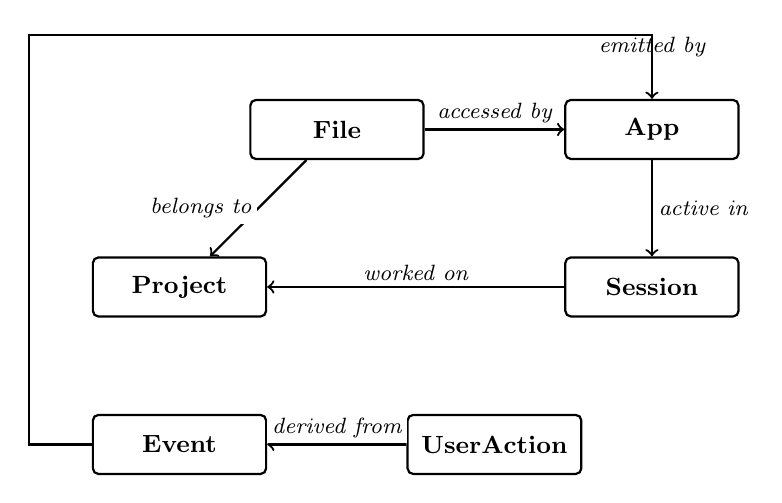
\begin{tikzpicture}[
	node/.style={
		draw, thick, rectangle, rounded corners=2pt,
		minimum width=2.2cm, minimum height=0.75cm,
		font=\small\bfseries, align=center, inner sep=5pt
	},
	edge/.style={->, thick},
	lbl/.style={font=\footnotesize\itshape, fill=white, inner sep=2pt},
	]
	
	\node[node] (file)    at (2.0,  4.0) {File};
	\node[node] (app)     at (6.0,  4.0) {App};
	\node[node] (project) at (0.0,  2.0) {Project};
	\node[node] (session) at (6.0,  2.0) {Session};
	\node[node] (event)   at (0.0,  0.0) {Event};
	\node[node] (action)  at (4.0,  0.0) {UserAction};
	
	\draw[edge] (file)    to node[lbl, above]      {accessed by}  (app);
	\draw[edge] (file)    to node[lbl, left]        {belongs to}   (project);
	\draw[edge] (app)     to node[lbl, right]       {active in}    (session);
	\draw[edge] (session) to node[lbl, above]       {worked on}    (project);
	\draw[edge] (event.west) -- ++(-0.8,0) -- ++(0,5.2)
	-| node[pos=0.75, above, font=\footnotesize\itshape] {emitted by} (app.north);
	\draw[edge] (action)  to node[lbl, above]       {derived from} (event);
	
\end{tikzpicture}
\caption{Knowledge Graph core schema. Nodes represent entities; edges
represent relationships. \texttt{Event} nodes are the lowest-level entries,
created directly from the event pipeline. \texttt{UserAction} nodes are
derived abstractions built from clusters of raw events.}
\label{fig:kg-schema}
\end{figure}

\subsection{Retention Policy}
\label{sec:retention}

The graph accumulates data indefinitely if left unchecked, which creates two
problems: storage grows, and the privacy surface area expands. The retention
policy defines how long data lives, with user control at every tier.

\begin{table}[htbp]
\caption{Knowledge Graph retention tiers}
\label{tab:retention}
\begin{tabularx}{\linewidth}{llX}
\toprule
\textbf{Tier} & \textbf{Default} & \textbf{Content} \\
\midrule
Raw eBPF events &
  30 days &
  High-volume, low-semantic-value syscall events. Already incorporated
  into higher-level nodes after ingestion; the raw records are largely
  redundant beyond the anomaly detection window. \\
Semantic nodes &
  12 months rolling &
  File, App, Session, and NetworkConnection nodes representing actual
  activity. This is where AI query value lives. Nodes past the window
  are summarized rather than deleted. \\
Pinned nodes &
  Permanent &
  Nodes explicitly marked by the user, active Project nodes, and nodes
  recently referenced in AI queries. Only manual deletion removes these. \\
\bottomrule
\end{tabularx}
\end{table}

\paragraph{Summarization.}
Hard deletion of aged nodes loses information abruptly. Instead, nodes past
the retention window are compacted into summary nodes that retain aggregate
statistics (access count, primary application, active period) while discarding
the individual event edges. The node still exists in the graph and AI queries
still find it; the granularity is reduced but the semantic content is
preserved. Summarization is triggered by access frequency rather than age: a
node that has not been queried in six months is a candidate regardless of when
it was created, while a node from two years ago that is queried regularly
remains granular. A background daemon identifies candidates nightly and
processes them during idle periods.

\paragraph{User controls.}
Settings exposes the retention window per tier with documented minimums, a
manual summarize-now option for specific time ranges, node and subgraph
deletion, full graph export for data portability, and storage usage broken down
by tier and time range. In managed deployments, administrators can set a
minimum retention for compliance-relevant audit events in a separate audit log,
but they cannot shorten the user's configured retention window for personal
graph data.
